% !TEX root = hw9-answers.tex
\chead{\textbf{Exercises week 9}}
\begin{document}
\flushleft\textbf{Topic: Structural Causal Models}
\section{The mysterious coin machine}

Consider the coin machine in Figure \ref{fig:coin_machine}.

\begin{figure}[H]
\centering
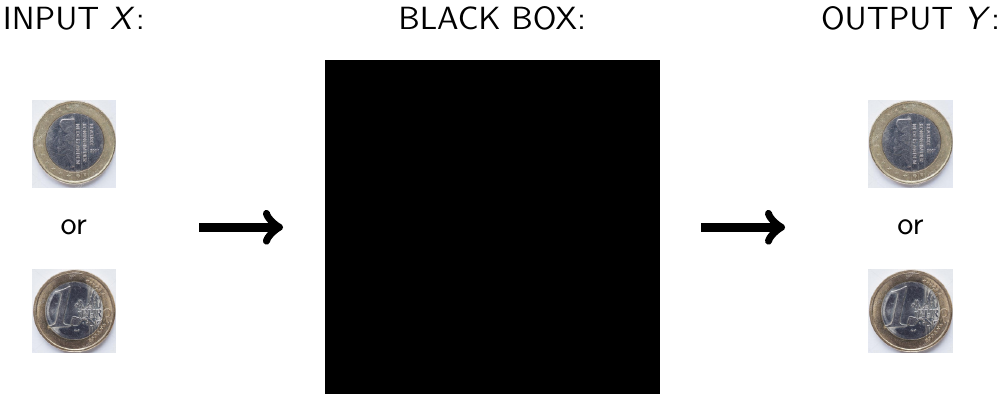
\includegraphics[width=1.0\textwidth]{blackbox}
\caption{The mysterious coin machine}
\label{fig:coin_machine}
\end{figure}

One can insert a coin with either heads or tails up (modeled as $X = +1$ and $X = -1$, respectively), and a few seconds later, it outputs the same coin, again with either heads or tails up (modeled as $Y = +1$ and $Y = -1$, respectively), i.e. the machine can flip the coin along the way. 
%Suppose you observe someone repeatedly inputting coins into the machine, which subsequently outputs each coin again with some orientation.
%You gather data from this observational distribution $P(X, Y)$.
You can conduct an experiment by inserting many coins into the machine and observing the outcomes. This leads you to collect data for the Markov kernel $P(Y | \text{do}(X))$.
After collecting lots of data and estimating both distributions based on them, you obtain the following Markov kernel:
\vspace{20pt}

\centerline{\begin{tabular}{cc|c}
    $x$ & $y$ & $P(Y = y | \text{do}(X = x))$ \\
\hline
-1    & -1 & 1/2  \\
-1 &  1 & 1/2  \\
\hline
1   & -1 & 1/2  \\
1 & 1 & 1/2 \\
\end{tabular}}
\vspace{15pt}
This seems like a rather boring machine. 
But, is it?

\begin{enumerate}
  \item Model the mysterious coin machine with two different SCMs $\mathcal{M}$ and $\widetilde{\mathcal{M}}$ whose observational Markov kernels agree with the one in the table above, and prove this agreement. Thereby, consider $X$ as an exogenous input variable and $Y$ as an endogenous variable.
    Construct the two SCMs in such a way that they will turn out to not be counterfactually equivalent (which you will then prove in the second part).  \textbf{(2pt)}
   
    \emph{Hint: Think of two different causal mechanisms, one which ignores the input orientation, and another one which makes use of it.}
  \item Prove that your two models $\mathcal{M}$ and $\widetilde{\mathcal{M}}$ are observationally and interventionally equivalent, but not counterfactually equivalent (with respect to $O = \{Y\}$). \textbf{(2pt)}
  \item Come up with a physical mechanism which could implement your causal models $\mathcal{M}$ and $\widetilde{\mathcal{M}}$ in the real world.  \textbf{(1pt)} 
  \end{enumerate}	


  \begin{gradedsolution}
    \begin{enumerate}
      \item We define $\mathcal{M} = \left\langle X, Y, W, \{-1,1\}^3, \text{Bernoulli}(1/2), f \right\rangle$ with 
	\begin{equation*}
	  f: \{-1,1\}^3 \to \{-1,1\}, \quad f(x, y, w) \coloneq w,
	\end{equation*}
	which simply outputs the coin in random orientation, independent of the input orientation.

	In contrast, we define $\widetilde{\mathcal{M}} = \left\langle X, Y, W, \{-1,1\}^3, \text{Bernoulli}(1/2), \widetilde{f} \right\rangle$, with the causal mechanism given by
	\begin{equation*}
	  \widetilde{f}: \{-1,1\}^3 \to \{-1,1\}, \quad \widetilde{f}(x, y, w) = x \cdot w,
	\end{equation*}
	which randomly decides whether to \emph{flip} the input orientation, and thus creates an output which depends functionally on the input.

	In order to show that the Markov kernels agree with the table, we first need the solution functions. 
	As can easily be checked, the unique solution functions are given by
	\begin{align*}
	  g: \{-1,1\}^2 \to \{-1,1\}, & \quad g(x, w) = w \\
	  \widetilde{g}: \{-1,1\}^2 \to \{-1,1\} & \quad g(x, w) = x \cdot w.
	\end{align*}
	Since they are unique, they define unique observational Markov kernels by Theorem 8.1.2, where we abbreviate the Bernoulli(1/2) distribution with $P$:
	\begin{align*}
	  g_{*}P(W | X): \mathcal{X}_X \dashrightarrow \mathcal{X}_Y, \quad (y | x) & \mapsto P\big(g^{-1}(y)_x\big) = P\big(\{w | w = g(w,x) = y\}\big) = \frac{1}{2} \\
	  \widetilde{g}_{*}P(W | X): \mathcal{X}_X \dashrightarrow \mathcal{X}_Y, \quad (y | x) & \mapsto P\left(\widetilde{g}^{-1}(y)_x\right) = P\left(\{w | x \cdot w = \widetilde{g}(w, x) = y \}\right) = P\left(y/x\right) = \frac{1}{2}.
	\end{align*}
	Note that by definition, we have $P_{\mathcal{M}}(Y | \text{do}(X)) = g_{*}P(W | X)$, and $P_{\widetilde{M}}(Y | \text{do}(X)) = \widetilde{g}_{*}P(W | X)$.
	Thus, we have proven $P_{\mathcal{M}}(Y = y | \text{do}(X = x)) = 1/2$ and $P_{\widetilde{M}}(Y = y | \text{do}(X = x)) = 1/2$ for all combinations of $x$ and $y$.
	This shows that the observational Markov kernels of our causal models agree with the table.
      \item Observational equivalence is precisely the statement that the observational Markov kernels agree, which holds since they both agree with the table.

	For interventional equivalence, note that we only need to show two observational equivalences: 
	That $\mathcal{M}_{\text{do}(\emptyset)}$ is observationally equivalent to $\widetilde{\mathcal{M}}_{\text{do}(\emptyset)}$ holds since intervention with the emptyset does not change the causal models.
	That $\mathcal{M}_{\text{do}(Y)}$ is observationally equivalent to $\widetilde{\mathcal{M}}_{\text{do}(Y)}$ holds trivially since $\mathcal{M}$ and $\widetilde{\mathcal{M}}$ differ only in their causal mechanism, and this is removed completely by making $Y$ an exogenous variable.

	Thus, we are only left with proving that these models are \emph{not} counterfactually equivalent. 
	For this, we explicitly construct the twinned SCMs:
	\begin{align*}
	  \mathcal{M}^{\text{twin}} = \left\langle \{X, X'\}, \{Y, Y'\}, W, \{-1,1\}^5, f \times f' \right\rangle, \ \ \text{with} \\
	  (f\times f')(x, x', y, y', w)  = (w, w) \in \{-1,1\}^2
	\end{align*}
	And:
	\begin{align*}
	  \widetilde{M}^{\text{twin}} = \left\langle \{X, X'\}, \{Y, Y'\}, W, \{-1,1\}^5, \widetilde{f} \times \widetilde{f}' \right\rangle, \ \ \text{with} \\
	  (\widetilde{f} \times \widetilde{f}')(x, x', y, y', w) = (x \cdot w, x' \cdot w) \in \{-1, 1\}^2.
	\end{align*}
	By definition, we need to show that they are not interventionally equivalent. 
	Since interventional equivalence includes observational equivalence, it is enough to show that they are not even observationally equivalent.
	Thus, let's construct their observational Markov kernels.
	The (obviously unique) solution functions are given by 
	\begin{align*}
	  g^{\text{twin}}: \{-1,1\}^3 \to \{-1,1\}^2, & \quad (x, x', w) \mapsto (w, w) \\
	  \widetilde{g}^{\text{twin}}: \{-1,1\}^3 \to \{-1,1\}^2, & \quad (x, x', w) \mapsto (x \cdot w, x' \cdot w).
	\end{align*}
	From this, we can construct the observational Markov kernels:
	\begin{align*}
	  g^{\text{twin}}_* P(W | X, X'): \ \ & \mathcal{X}_{\{X,X'\}} \dashrightarrow \mathcal{X}_{\{Y,Y'\}} \\
	  (y, y' | x, x') & \mapsto P\left((g^{\text{twin}})^{-1}(y, y')_{(x,x')}\right) \\
	  & = P\left(\{w | (w,w) = g^{\text{twin}}(x, x', w) = (y, y')\right) \\
	    & = \begin{cases} 0, \ \ \ y \neq y' \\ 1/2, \ \ \ \text{else}.\end{cases}
	\end{align*}
	And:
	\begin{align*}
	\widetilde{g}^{\text{twin}}_* P(W | X, X'): \ \  & \mathcal{X}_{\{X,X'\}} \dashrightarrow \mathcal{X}_{Y,Y'\}} \\
	 (y, y' | x, x') & \mapsto P\left((\widetilde{g}_{\text{twin}})^{-1}(y,y')_{(x,x')}\right) \\
	 & = P\left(\{w | (x \cdot w, x' \cdot w) = \widetilde{g}^{\text{twin}}(x, x', w) = (y, y')\}\right) \\
	  & = P\left(\{w | y/x = w = y'/x'\right) \\
	    & = \begin{cases} 0, \ \ \ y/x \neq y'/x' \\ 1/2, \ \ \ \text{else}.\end{cases}
	\end{align*}
	These are simply not the same Markov kernels, which can be seen for example in the case $y = y'$ and $x \neq x'$, which proves the claim that they are not counterfactually equivalent.

	\textbf{Addendum:} To get some more intuitions, we now express the difference of the Markov kernels using counterfactual distributions.
	For this, set 
	\begin{align*}
	  P_{\mathcal{M}}(Y, Y' | \text{do}(X), \text{do}(X')) & \coloneq g_{*}^{\text{twin}}P(W | X, X'), \text{ and } \\
	  P_{\widetilde{\mathcal{M}}}(Y, Y' | \text{do}(X), \text{do}(X')) & \coloneq  \widetilde{g}_*^{\text{twin}}P(W | X, X').
	\end{align*}
	Counterfactual distributions are then expressed by conditioning the Markov kernels on $Y$, i.e. on the ``original outcome''.
	In the case $y = y'$ and $x \neq x'$, we then obtain:
	\begin{align*}
	  P_{\mathcal{M}}(Y' = y' | Y = y, \doit(X = x), \doit(X' = x')) & = \frac{P_{\mathcal{M}}(Y' = y', Y = y | \doit(X = x), \doit(X' = x'))}{P_{\mathcal{M}}(Y = y | \doit(X = x) \doit(X ' = x'))} \\
	  & = \frac{1/2}{P_{\mathcal{M}}(Y = y | \doit(X = x))} \\
	  & = \frac{1/2}{1/2} \\
	  & = 1.
	\end{align*}
	In the second step, we have used that the marginal Markov kernel in which $Y'$ is ``marginalized out'' does not depend on $X'$ anymore, as can easily be shown in general such situations. 
	Similarly, one can show that $P_{\widetilde{\mathcal{M}}}(Y' = y' | Y = y, \doit(X = X), \doit(X' = x')) = 0$.
	Thus, the counterfactual distributions are different.

	This is the expected outcome: The first model does not care about the input at all, and so if the ``randomness'' $w$ is the same in the actual, and the counterfactual world, then the outcome $y = y'$ is the same.
	However, the second model multiplies the ``randomness'' $w$ with the input $x$ or $x'$, and so if the input changes, the output also must change, and so we cannot have the outcome $y' = y$.

	
      \item $\mathcal{M}$ could be implemented physically by tossing a second coin internally, and then orienting the coin which was input in accordance to the internal coin toss.

	$\widetilde{\mathcal{M}}$ can be implemented by tossing a second coin internally, and then flipping the coin which was input based on the result of the internal coin toss.

	Assuming that the internal coin toss happens each time already before the coin is put in, this means that it is already pre-determined whether the coin will come out heads or tails (implementation 1) or whether it will be flipped along the way (second model), meaning that the twinned SCM models counterfactuals correctly.

      \end{enumerate}
  \end{gradedsolution}


\section{Stability of equivalences by different operations}

Prove the following remarks on the equivalence of SCMs from the lecture:

\begin{enumerate}
  \item Prove that equivalence of SCMs ($\mathcal{M} \equiv \widetilde{\mathcal{M}}$) is indeed an equivalence relation.  \textbf{(1pt)}
  \item Equivalence is preserved by hard interventions, i.e.: if $\mathcal{M}$ is equivalent to $\widetilde{\mathcal{M}}$ and $T \subseteq J \cup V \cup W$ is an intervention target, then $\mathcal{M}_{\doit(T\dots)}$ is equivalent to $\widetilde{\mathcal{M}}_{\doit(T\dots)}$. Do this for the three variants of hard interventions.  \textbf{(2pt)}
  \item Equivalence is preserved by twinning. \textbf{(1pt)}  
  \item Show that equivalent SCMs have the same solution functions. 
    Deduce from this and from Exercise 2.2 that unique solvability and simplicity are invariants of equivalence, i.e.: 
    If $\mathcal{M}$ is equivalent to $\widetilde{\mathcal{M}}$ and $\mathcal{M}$ is uniquely solvable or simple, then $\widetilde{\mathcal{M}}$ is also uniquely solvable or simple, respectively. \textbf{(2pts)} 
  \item Equivalent SCMs have the same solutions and outcomes for a specified input (Definition 4.6.3), the same solutions (Definition 4.6.5), and the same Markov kernels (Definition 5.5.1). \textbf{(2pts)} 
  \end{enumerate}


  \begin{gradedsolution}
    In all parts we assume that $\mathcal{M} = \left\langle J, V, W, \mathcal{X}, P, f \right\rangle$ and $\widetilde{M} = \left\langle J, V, W, \mathcal{X}, P, \widetilde{f} \right\rangle$ are two SCMs which can only differ in their causal mechanisms.
    \begin{enumerate}
    \item This follows directly from the fact that logical equivalence ``$\Longleftrightarrow$'' is an equivalence relation. 
    \item We discuss only the case of hard interventions with specified target value, since the other two cases work the same way (and are even slightly easier to show).
      Thus, let $T \subseteq J \cup V \cup W$ be an intervention target and $\xi_{T} \in \mathcal{X}_T$ be the intervention target value. 
      The intervened SCMs are then given by 
      \begin{align*}
	\mathcal{M}_{\text{do}(X_T = \xi_T)} = \left\langle J \setminus T, V \cup T, W \setminus T, \mathcal{X}, P_{W \setminus T}, (f_{V \setminus T}, \xi_T) \right\rangle, \\
	\widetilde{\mathcal{M}}_{\text{do}(X_T = \xi_T)} = \left\langle J \setminus T, V \cup T, W \setminus T, \mathcal{X}, P_{W \setminus T}, (\widetilde{f}_{V \setminus T}, \xi_T) \right\rangle.
      \end{align*}
      Now, set $f' \coloneq (f_{V \setminus T}, \xi_T)$ and $\widetilde{f}' \coloneq (\widetilde{f}_{V \setminus T}, \xi_T)$. 

      Then, for $v \in V \setminus T$ and arbitrary $x \in \mathcal{X}$ we obtain:
      \begin{align*}
	x_v = f'_v(x) & \Longleftrightarrow x_v = f_v(x) \\
	& \Longleftrightarrow x_v = \widetilde{f}_v(x) \\
	& \Longleftrightarrow x_v = \widetilde{f}'_v(x).
      \end{align*}
      Thereby, in the first step we used the definition of $f'$ and that $v \in V \setminus T$. 
      In the second step, we used the equivalence $\mathcal{M} \equiv \widetilde{\mathcal{M}}$.
      In the last step, we used the definition of $\widetilde{f}'$ and again that $v \in V \setminus T$.

      Finally, for $v \in T$ and arbitrary $x \in X$, we obtain:
      \begin{align*}
	x_v = f'_v(x) & \Longleftrightarrow x_v = \xi_v \\
	& \Longleftrightarrow x_v = \widetilde{f}'_v(x).
      \end{align*}
      Since $V \cup T = (V \setminus T) \cup T$, this proves the claim.
    \item Let $\mathcal{M} \equiv \widetilde{\mathcal{M}}$.
      Let the twinned SCMs be given by
      \begin{align*}
	\mathcal{M}^{\text{twin}} & = \left\langle J \cup J', V \cup V', W, \mathcal{X}^{\text{twin}}, P, f \times f' \right\rangle \\
	\widetilde{\mathcal{M}}^{\text{twin}} & = \left\langle J \cup J', V \cup V', W, \mathcal{X}^{\text{twin}}, P, \widetilde{f} \times \widetilde{f}' \right\rangle,
      \end{align*}
      where we set $\mathcal{X}^{\text{twin}} = \mathcal{X}_J \times \mathcal{X}_{J} \times \mathcal{X}_{V} \times \mathcal{X}_V \times \mathcal{X}_W$, and where $f \times f'$ is given by 
      \begin{equation*}
	(f \times f')(x_J, x_{J'}, x_V, x_{V'}, x_W) = (f(x_J, x_V, x_W), f(x_{J'}, x_{V'}, x_W)) \in \mathcal{X}_V \times \mathcal{X}_{V}.
      \end{equation*}
      $\widetilde{f} \times \widetilde{f}'$ is constructed in the same way. 
      
      Then, for arbitrary $v \in V$ and $x \in \mathcal{X}^{\text{twin}}$ we obtain:
      \begin{align*}
	x_v = (f \times f')_v(x_J, x_{J'}, x_V, x_{V'}, x_W) & \Longleftrightarrow x_v = f_v(x_J, x_V, x_W) \\
	& \Longleftrightarrow x_v = \widetilde{f}_v(x_J, x_V, x_W) \\
	& \Longleftrightarrow x_v = (\widetilde{f} \times \widetilde{f}')(x_J, x_{J'}, x_V, x_{V'}, x_W).
      \end{align*}
      The same arguments work if $v \in V'$, and thus we are done and have shown that the twinned SCMs are still equivalent.
    \item 

      Let $\mathcal{M} \equiv \widetilde{\mathcal{M}}$, and let $g: \mathcal{X}_J \times \mathcal{X}_W \to \mathcal{X}_V$ be any measurable function.
      Then the following equivalences hold:
      \begin{align*}
	g \text{ is a solution function for } \mathcal{M} & \Longleftrightarrow \forall x_J, \forall x_W: \ \ g(x_J, x_W) = f(x_J, g(x_J, x_W), x_W) \\
	&   \Longleftrightarrow \forall v, \forall x_J, \forall x_W: \ \ g_v(x_J, x_W) = f_v(x_J, g(x_J, x_W), x_W) \\
	&  \Longleftrightarrow   \forall v, \forall x_J, \forall x_W: \ \ g_v(x_J, x_W) = \widetilde{f}_v(x_J, g(x_J, x_W), x_W) \\
	& \Longleftrightarrow   \forall x_J, \forall x_W: \ \ g(x_J, x_W) = \widetilde{f}(x_J, g(x_J, x_W), x_W) \\
	& \Longleftrightarrow g \text{ is a solution function for } \widetilde{\mathcal{M}}.
      \end{align*}
      This shows that equivalent SCMs have the same solution functions, and consequently that unique solvability is an invariant of equivalence.

      Now, assume that $\mathcal{M}$ is simple and that $\mathcal{M} \equiv \widetilde{\mathcal{M}}$.
      We want to show that $\widetilde{\mathcal{M}}$ is also simple.
      For this, let $T \subseteq J \cup V \cup W$ be any subset.
      Then we need to show that $\widetilde{\mathcal{M}}_{\text{do}(T)}$ is uniquely solvable.
      But note that due to the simplicity of $\mathcal{M}$, $\mathcal{M}_{\text{do}(T)}$ is uniquely solvable. 
      Furthermore, as was shown in Exercise 2.2, $\mathcal{M}_{\text{do}(T)} \equiv \widetilde{\mathcal{M}}_{\text{do}(T)}$.
      We have just shown that unique solvability is an invariant of equivalence, and thus the unique solvability of $\widetilde{\mathcal{M}}_{\text{do}(T)}$ automatically follows.

    \item Let $\mathcal{M} \equiv \widetilde{\mathcal{M}}$.
      Let $X_{V\cup W}^{\text{do}(x_J)}$ be any random variable with codomain $\mathcal{X}_V \times \mathcal{X}_W$, and with $x_J \in \mathcal{X}_J$.
      We trivially have the following equivalences:
      \begin{align*}
      &	X_{V \cup W}^{\text{do}(x_J)} \text{ is a solution for } \mathcal{M} \text{ with input } x_J \in \mathcal{X}_J \\
      \Longleftrightarrow & X_W^{\text{do}(x_J)} \sim P \text{ and } X_V^{\text{do}(x_J)} = f(x_J, X_V^{\text{do}(x_J)}, X_W^{\text{do}(x_J)}) \text{ a.s. } \\
      \Longleftrightarrow & X_W^{\text{do}(x_J)} \sim P \text{ and } \forall v \in V: \ \ X_v^{\text{do}(x_J)} = f_v(x_J, X_V^{\text{do}(x_J)}, X_W^{\text{do}(x_J)}) \text{ a.s. } \\
      \Longleftrightarrow & X_W^{\text{do}(x_J)} \sim P \text{ and } \forall v \in V: \ \ X_v^{\text{do}(x_J)} = \widetilde{f}_v(x_J, X_V^{\text{do}(x_J)}, X_W^{\text{do}(x_J)}) \text{ a.s. } \\
      \Longleftrightarrow & X_W^{\text{do}(x_J)} \sim P \text{ and } X_V^{\text{do}(x_J)} = \widetilde{f}(x_J, X_V^{\text{do}(x_J)}, X_W^{\text{do}(x_J)}) \text{ a.s. } \\
      \Longleftrightarrow  &	X_{V \cup W}^{\text{do}(x_J)} \text{ is a solution for } \widetilde{\mathcal{M}} \text{ with input } x_J \in \mathcal{X}_J. 
      \end{align*}
      This shows that equivalent SCMs have the same solutions with specified inputs.
      Since (potential) outcomes with specified inputs are, by definition, just the observed parts of solutions with specified inputs, this also shows that equivalent SCMs have the same (potential) outcomes with specified solutions.
      
      From this, one can immediately deduce that equivalent SCMs also have the same solutions (without specified input) and Markov kernels.
    \end{enumerate}
  \end{gradedsolution}

  \section{The Ladder of Causation}

  In this exercise, we prove parts of the ``Ladder of Causation'', which, roughly speaking, comes down to the insight that modeling interventions is more expressive than just modeling observations, and that modeling counterfactuals is more expressive than just modeling interventions.
  All of this is Proposition 8.3.8 in the lecture notes.

  Let $\mathcal{M}$ and $\widetilde{\mathcal{M}}$ be two simple SCMs and $O \subseteq (V \cap \widetilde{V}) \cup (W \cap \widetilde{W})$. 
  Prove the following:
  \begin{enumerate}
    \item If $\mathcal{M} \equiv \widetilde{\mathcal{M}}$ then $\mathcal{M}$ and $\widetilde{\mathcal{M}}$ are counterfactually equivalent with respect to $O$.  \textbf{(1pt)}
    \item If $\mathcal{M}$ and $\widetilde{\mathcal{M}}$ are interventionally equivalent with respect to $O$, then $\mathcal{M}$ and $\widetilde{\mathcal{M}}$ are observationally equivalent with respect to $O$.   \textbf{(1pt)} 
    \end{enumerate}
    As you see, we have left out the middle part of the ladder, which is about proving that counterfactual equivalence implies interventional equivalence. 
    The reason is that that part is relatively inconvenient to prove without more knowledge on solution functions and Markov kernels of twinned SCMs.
    However, if you wish, you can give it a try.
  \begin{gradedsolution}
    \begin{enumerate}
      \item Assume $\mathcal{M} \equiv \widetilde{\mathcal{M}}$.
	By Exercise 2.3, we can deduce $\mathcal{M}^{\text{twin}} \equiv \widetilde{\mathcal{M}}^{\text{twin}}$.
	From Exercise 2.2, we obtain $\left( \mathcal{M}^{\text{twin}}\right)_{\doit(T)} \equiv \left( \widetilde{\mathcal{M}}^{\text{twin}}\right)_{\doit(T)} $ for all $T \subseteq J \cup J' \cup V \cup V' \cup W$.
	This then also holds for all $T \subseteq O \cup O'$.
	From Exercise 2.5, we then obtain that, for all these $T$, $\left( \mathcal{M}^{\text{twin}}\right)_{\doit(T)} $ and $\left( \widetilde{\mathcal{M}}^{\text{twin}}\right)_{\doit(T)} $ have the same Markov kernels.
	Marginalizing these Markov kernels, and only keeping the variables $X_{O \cup O' \setminus T}$ in them, this implies observational equivalence of $\left( \mathcal{M}^{\text{twin}}\right)_{\doit(T)} $ $\left( \widetilde{\mathcal{M}}^{\text{twin}}\right)_{\doit(T)} $ with respect to $O \cup O' \setminus T$.
	Since this holds for all $T \subseteq O \cup O'$, this implies interventional equivalence of $\mathcal{M}^{\text{twin}}$ and $\widetilde{\mathcal{M}}^{\text{twin}}$ with respect to $O \cup O'$.
	This, in turn, is counterfactual equivalence of $\mathcal{M}$ and $\widetilde{\mathcal{M}}$ with respect to $O$.
	Thus, we are done.
	  \item That $\mathcal{M}$ and $\widetilde{\mathcal{M}}$ are interventionally equivalent with respect to $O$ means that, for all $T \subseteq O$, $\mathcal{M}_{\text{do}(T)}$ is observationally equivalent to $\widetilde{\mathcal{M}}_{\text{do}(T)}$ with respect to $O \setminus T$.
	    Setting $T = \emptyset$ implies that $\mathcal{M}$ and $\widetilde{\mathcal{M}}$ are observationally equivalent with respect to $O$.
      \end{enumerate}
  \end{gradedsolution}
\end{document}
